\documentclass{deliverablereport}

\deliverable{component-architecture}{hpc-configure}
\deliverydate{XX/YY/201Z}
\duedate{31/08/2019 (M48)}
\author{Author names}

\newcommand{\fflasffpack}{\textsc{fflas-ffpack}\xspace}
\begin{document}
\maketitle
% This will be the abstract, fetched from the github description
\githubissuedescription

% write the report here


%%%%%%%%%%%%%%%%%%%%%%%%%%%%%%%%%%%%%%%%%%%%%%%%%%%%%%%%%%%%%%
\section{Introduction}

%%%%%%%%%%%%%%%%%%%%%%%%%%%%%%%%%%%%%%%%%%%%%%%%%%%%%%%%%%%%%%
\section{Number Theory}

PARI-MT and the difficulty of composing a threaded systems into another.

%%%%%%%%%%%%%%%%%%%%%%%%%%%%%%%%%%%%%%%%%%%%%%%%%%%%%%%%%%%%%%
\section{Finite field linear algebra}

Finite field linear algebra is a core building block in computational mathematics and deliver high computing throughput
to a wide range of applications, including number theory, group theory, combinatorics, etc. \SageMath relies on the
\fflasffpack library for its critical linear algebra operations on prime fields of less than 23 bits and consequently
also for numerous computations with multiprecision integer matrices.  

The \fflasffpack library had some preliminary support for multi-core parallelism for matrix
multiplication and Gaussian elimination.
Instead of being tight to a specific parallel language, the library uses a Domain Specific Language, Paladin~\cite{},
to provide the library programmer with unique API for writing parallel code, which is then translated into 
OpenMP~\cite{}, Cilk~\cite{}, Intel-TBB~\cite{}, or XKaapi~\cite{} directives.


\begin{figure}[htb]
  \begin{center}
    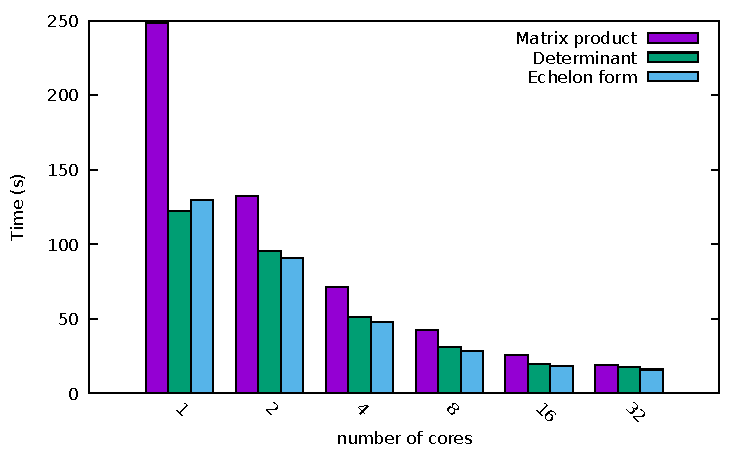
\includegraphics[width=.8\textwidth]{Pictures/histo_bigfoot3}
    \caption{Parallel speedup for some finite field linear algebra operations in SageMath}
  \end{center}
\end{figure}


\end{document}

%%% Local Variables:
%%% mode: latex
%%% TeX-master: t
%%% End:

